\documentclass[aspectratio=43,english]{beamer} %If you want to create Polish presentation, replace 'english' with 'polish' and uncomment 3-th line, i.e., '\usepackage{polski}'
\usepackage[utf8]{inputenc}
\usepackage{polski} %Uncomment for Polish language
\usepackage{babel}
\usepackage{listings} %We want to put listings

\mode<beamer>{ 	%in 'beamer' mode
	\hypersetup{pdfpagemode=FullScreen}		%Enable Full screen mode
	\usetheme{JuanLesPins} 		%Show part title in right footer
	%\usetheme[dark]{AGH}                 		%Use dark background
	%\usetheme[dark,parttitle=leftfooter]{AGH}  	%Use dark background and show part title in left footer
}
\mode<handout>{	%in 'handout' mode
	\hypersetup{pdfpagemode=None}		
	\usepackage{pgfpages}
  	\pgfpagesuselayout{4 on 1}[a4paper,border shrink=5mm,landscape]	%show 4 slides on 1 page
  	\usetheme{boxes}
  	\addheadbox{structure}{\quad\insertpart\hfill\insertsection\hfill\insertsubsection\qquad} 	%content of header
 	\addfootbox{structure}{\quad\insertauthor\hfill\insertframenumber\hfill\insertsubtitle\qquad} 	%content of footer
}

\AtBeginPart{ %At begin part: display its name
	\frame{\partpage}
} 


%%%%%%%%%%% Configuration of the listings package %%%%%%%%%%%%%%%%%%%%%%%%%%
% Source: https://en.wikibooks.org/wiki/LaTeX/Source_Code_Listings#Using_the_listings_package
%%%%%%%%%%%%%%%%%%%%%%%%%%%%%%%%%%%%%%%%%%%%%%%%%%%%%%%%%%%%%%%%%%%%%%%%%%%%
\lstset{ %
  backgroundcolor=\color{white},   % choose the background color
  basicstyle=\footnotesize,        % the size of the fonts that are used for the code
  breakatwhitespace=false,         % sets if automatic breaks should only happen at whitespace
  breaklines=true,                 % sets automatic line breaking
  captionpos=b,                    % sets the caption-position to bottom
  commentstyle=\color{green},      % comment style
  deletekeywords={...},            % if you want to delete keywords from the given language
  escapeinside={\%*}{*)},          % if you want to add LaTeX within your code
  extendedchars=true,              % lets you use non-ASCII characters; for 8-bits encodings only, does not work with UTF-8
  frame=single,	                   % adds a frame around the code
  keepspaces=true,                 % keeps spaces in text, useful for keeping indentation of code (possibly needs columns=flexible)
  keywordstyle=\color{blue},       % keyword style
  morekeywords={*,...},            % if you want to add more keywords to the set
  numbers=left,                    % where to put the line-numbers; possible values are (none, left, right)
  numbersep=5pt,                   % how far the line-numbers are from the code
  numberstyle=\tiny\color{gray},   % the style that is used for the line-numbers
  rulecolor=\color{black},         % if not set, the frame-color may be changed on line-breaks within not-black text (e.g. comments (green here))
  showspaces=false,                % show spaces everywhere adding particular underscores; it overrides 'showstringspaces'
  showstringspaces=false,          % underline spaces within strings only
  showtabs=false,                  % show tabs within strings adding particular underscores
  stepnumber=2,                    % the step between two line-numbers. If it's 1, each line will be numbered
  stringstyle=\color{cyan},        % string literal style
  tabsize=2,	                   % sets default tabsize to 2 spaces
  title=\lstname,                  % show the filename of files included with \lstinputlisting; also try caption instead of title
                                   % needed if you want to use UTF-8 Polish chars
  literate={?}{{\k{a}}}1
           {?}{{\k{A}}}1
           {?}{{\k{e}}}1
           {?}{{\k{E}}}1
           {�}{{\'o}}1
           {�}{{\'O}}1
           {?}{{\'s}}1
           {?}{{\'S}}1
           {?}{{\l{}}}1
           {?}{{\L{}}}1
           {?}{{\.z}}1
           {?}{{\.Z}}1
           {?}{{\'z}}1
           {?}{{\'Z}}1
           {?}{{\'c}}1
           {?}{{\'C}}1
           {?}{{\'n}}1
           {?}{{\'N}}1
}
%%%%%%%%%%%%%%%%%


\title{Metody Obliczeniowe w Nauce i Technice}
\author{Marian Bubak, PhD}
\date{}
\institute[AGH]{
	Institute of Computer Science\\ul. Kawiory 21\\30-055 Krakow\\
	Poland\\
	\url{http://www.icsr.agh.edu.pl/~mownit/}
}



%%%%%%%%%%%%%%%%
\usepackage{amsmath}
\usepackage{amssymb}
%%%%%%%%%%%%%%%%

\subtitle{17 - Minimalizacja funkcji}
\setcontributors{Anna Bukowska\\Yurii Vyzhha\\Arkadiusz Placha}

\AtBeginSection[]{
  \begin{frame}
  \vfill
  \centering
  \begin{beamercolorbox}[sep=8pt,center,shadow=true,rounded=true]{title}
    \usebeamerfont{title}\insertsectionhead\par%
  \end{beamercolorbox}
  \vfill
  \end{frame}
}

\begin{document}
  	\maketitle
	%%%%%%%%%%%%%%%%
	\begin{frame}[allowframebreaks]{Plan wykładu}
		\tableofcontents
	\end{frame}
	%%%%%%%%%%%%%%%%
	\section{Wstęp}

\subsection{Motywacja}

  \begin{frame}{Motywacja}
    Szeroka klasa zagadnień -- szukanie najmniejszej wartości
    przyjmowanej przez funkcję jednej lub wielu zmiennych.

    \begin{exampleblock}{Przykład}
      \begin{itemize}
        \item minimalizacja kosztów produkcji
        \item \ldots
        \item linia geodezyjna w ogólnej teorii względności
      \end{itemize}
    \end{exampleblock}
  \end{frame}

  \begin{frame}{Motywacja}
    \begin{exampleblock}{Przykład cd.}
      \begin{itemize}
        \item przykład klasyczny:\\
        \textbf{estymacja} parametrów modelu teoretycznego
        przez \textbf{minimalizację} różnicy między danymi
        teoretycznymi a eksperymentalnymi:\\
        $
          min!F(x) = \sum_{k = 1}^{n} \left[ \frac{Y_k - T_k(\vec x)}{\sigma_k}
          \right] ^2 Y_k \text{-- zmierzone wartości,}
        $ \\
        $ \sigma_k $ - błąd pomiaru,\\
        $ T_k $ - wartości teoretyczne, zależne od parametrów~
        $ x_i{,}\ i=1{,} \dots {,}n $ \\
        $ K \geq n{,}\ \text{zwykle}\ K \gg n $
      \end{itemize}
    \end{exampleblock}
  \end{frame}

\subsection{Terminologia}

  \begin{frame}{Terminologia}
    \begin{block}{Terminologia}
      \begin{itemize}
        \item tradycyjnie: \textbf{minimalizacja}
        \item maksymalizacja $(F = -f(x))$
        \item optymalizacja -- kolizja z metodą teorii
        sterowania, (oparta o rachunek wariacyjny)
        \item b. stary termin: programowanie (liniowe,
        nieliniowe, matematyczne)
        \item ekstremalizacja
        \item hill-climbing \\
        \textbf{function minimalization !!!}
      \end{itemize}
    \end{block}
  \end{frame}

\subsection{Zdefiniowanie zagadnienia}

  \begin{frame}{Zdefiniowanie zagadnienia}
    \begin{block}{Zdefiniowanie zagadnienia}
      \textbf{Mając daną funkcję $ F(x) $ znaleźć wartość
      zmiennej $ x $, dla której $ F(x) $ przyjmuje
      najmniejszą wartość, przy czym:}
      \begin{enumerate}
        \item $ F(x) $ nie musi być zadana analitycznie --
        tylko: dla każdego $ x $ znamy jej wartość $ F(x) $
        \item wartości $ x $ mogą być ograniczone do pewnego
        obszaru -- constrained minization
        \item mogą być dostępne $ \frac{\partial F}{\partial x} $
        \item $ f(x) $ jest obliczana w wielu punktach --
        aż do osiągnięcia minimum. ($ F(x) $ -- to procedura)
      \end{enumerate}
    \end{block}
  \end{frame}

  \begin{frame}{Zdefiniowanie zagadnienia}
    \begin{block}{Najlepsza metoda -- taka, która:}
      \begin{itemize}
        \item znajduje minimum (z zadaną tolerancją)
        po najmniejszej liczbie obliczeń funkcji
        \item ma małą złożoność obliczeniową (sama
        metoda)
        \item wymaga mało pamięci
      \end{itemize}
    \end{block}
  \end{frame}

\subsection{Gdzie szukać minimum funkcji? (global minimum)}

  \begin{frame}{Gdzie szukać minimum funkcji? (global minimum)}
    \begin{block}{$ F(x) $ przyjmuje minimum w jednym z punktów:}
      \begin{enumerate}
        \item wszystkie $ \frac{\partial F}{\partial x} = 0 $
        (p. stacjonarny -- stationary point)
        \item niektóre $ \frac{\partial F}{\partial x} $
        nie istnieją (wierzchołek -- cusp)
        \item na krawędzi obszaru (edge point)
      \end{enumerate}
    \end{block}
    Gdy nie znamy funkcji analitycznie -- musimy ograniczyć
    się do minimum lokalnego $ x_0 $:
    \begin{displaymath}
      \forall x \in \text{otoczenia}\ x_0{,}\ F(x) > F(x_0)
      \to \text{\emph{unconstrained local minimization}}
    \end{displaymath}
  \end{frame}

\subsection{Kształt funkcji $ F(x) $}
  \begin{frame}{Kształt funkcji $ F(x) $}
    \begin{block}{Założenie}
      $ F(x) $ -- ma sens fizyczny $ \Rightarrow $ w rozpatrywanym
      obszarze istnieją jej wszystkie pochodne.
    \end{block}
    Wokół $ x_1 - F(x) $ -- \textbf{w szereg Taylora (1-D):}
    \begin{displaymath}
      F(x) = F(x_1) + \left. \frac{\partial F}{\partial x} \right|_{x_1}(x - x_1) +
      \left. \frac{1}{2} \frac{\partial^2 F}{\partial x^2} \right|_{x_1}(x - x_1)^2 +
      \dots
    \end{displaymath}
    \begin{itemize}
      \item a priori nie znamy obszaru jego zbieżności
      \item im mniejsza $ (x - x_1) $ - tym mniej ważne człony
      wyższych rzędów
    \end{itemize}
    $ \Rightarrow $ dla małych kroków -- przewidywania oparte
    na wyrazach niższego rzędu powinny być wystarczające.

  \end{frame}

  \begin{frame}{Kształt funkcji $ F(x) $}
    dla n-D: $ x \to \vec{x} $
    \begin{displaymath}
      F(\vec{x}) = \underbrace{F(\vec{x_1})}_{\text{stały}} +
      \vec{g}^T * (\vec{x} - \vec{x_1}) +
      \frac{1}{2}(\vec{x} - \vec{x_1})^T * G * (\vec{x} - \vec{x_1}) + \dots
    \end{displaymath}
    \begin{displaymath}
      g_i = \left. \frac{\partial F}{\partial x} \right|_{\vec{x_1}} \text{-- gradient;}\quad
      G_{ij} = \left. \frac{\partial^2 F}{\partial x_i \partial y_j} \right|_{\vec{x_1}}
    \end{displaymath}
    symbole $ \Rightarrow $ ($ x_i $ -- składowa; $ \vec{x_i} $
    -- wektor; niekiedy zamiast $ \vec{x} $ -- samo~$ x $)

  \end{frame}

  \begin{frame}{Kształt funkcji $ F(x) $}
    $ \vec{g}^T * (\vec{x} - \vec{x_1}) $ -- proporcjonalny do
    gradientu, wskazuje kierunek największego spadku funkcji,
    w pobliżu minimum: $ \vec{g} \to 0{,}\ (\vec{x} - \vec{x_1}) \to 0
    \; \Rightarrow $ człon liniowy, nie przepowiada minimum,
    nie można go użyć do określenia wielkości kroku.
    $ \frac{1}{2}((\vec{x} - \vec{x_1})^T) * G * (\vec{x} - \vec{x_1}) $
    -- kwadratowy, najniższy człon przydatny do przewidywania minimum
    $ G \approx $ stale w małych obszarach
    \begin{alertblock}{Uwaga}
      Ta analiza nie jest słuszna dla $ F(\vec{x}) $ liniowych
      od $ \vec{x} $;\\
      \textbf{Wtedy:} programowanie liniowe, rozwiązanie --
      krawędzi obszaru ograniczeń.
    \end{alertblock}
  \end{frame}

  \begin{frame}{Kształt funkcji $ F(x) $}
    \begin{block}{Optymalne algorytmy minimalizacji}
      Nie ma uniwersalnej metody minimalizacji. Dla b.~złego
      algorytmu można znaleźć $ F(x) $, którą minimalizuje on
      najszybciej -- i~odwrotnie.\\
      \textbf{Zasada:} dobór algorytmu do funkcji.

    \end{block}

  \end{frame}

 	%%%%%%%%%%%%%%%%%%%%%%%
	\section{Minimalizacja w 1-D}
  \begin{frame}{Minimalizacja w 1-D}
    \begin{block}{Przydatność metod 1-D dla zag. n-D}
      \begin{itemize}
        \item prosta ilustracja ogólnych problemów
        \item metody 1-D -- często: element składowy metod n-D

      \end{itemize}

    \end{block}

  \end{frame}

\subsection{Przeglądanie siatki (grid search)}
  \begin{frame}{Przeglądanie siatki \emph{(grid search)}}
    % \centering
    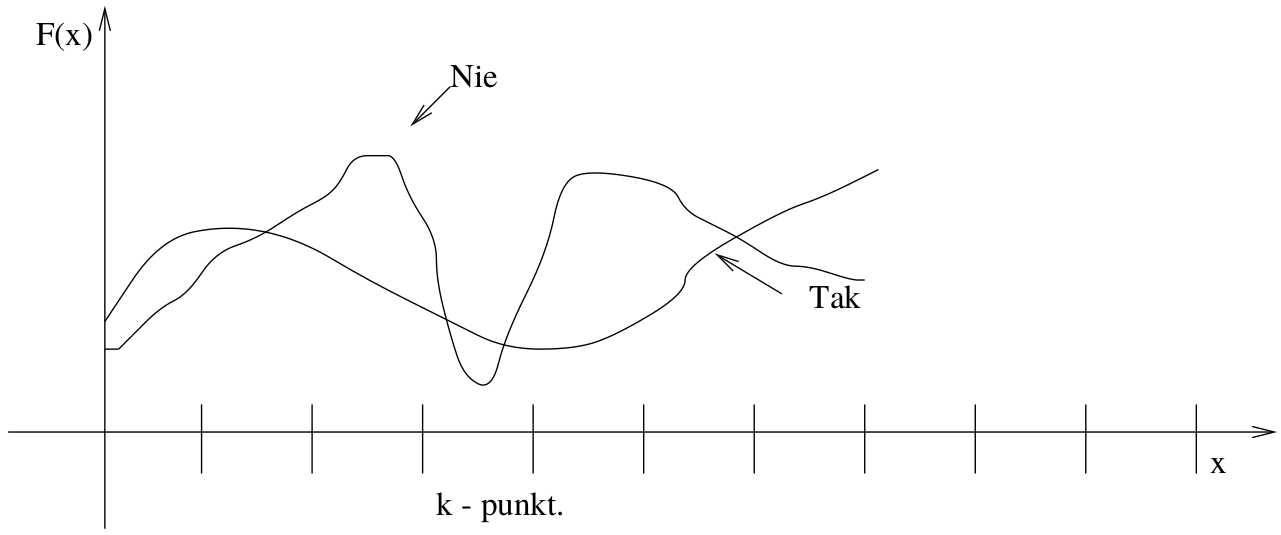
\includegraphics[width=1\textwidth]{img/17/przegladanie_siatki}
  \end{frame}

  \begin{frame}{Przeglądanie siatki \emph{(grid search)}}
    \begin{block}{Realizacja}
      \begin{itemize}
        \item przegląd wartości
        \item wybór najmniejszej $ \to $ odległości od minimum
        $ 0 \leq \frac{\Delta x}{2} $
      \end{itemize}
    \end{block}
    \begin{block}{Wady}
      \begin{itemize}
        \item nie może być stosowana dla $ \infty $ przedziału
        \item nieefektywna $ \to $ nie "uczy się" własności funkcji % był przecinek pred "własności"
      \end{itemize}
    \end{block}
  \end{frame}

  \begin{frame}{Przeglądanie siatki \emph{(grid search)}}
    \begin{tabular}{@{} c l c c c @{}}
      & $ 100 $ & punktów & w & 1 -- D \\
      $ \Rightarrow $ Zawężenie obszaru do 1\% $ \Rightarrow $ & $ 100^{2} $ & & w & 2 -- D \\
      & $ 100^{10} $ & & w & 10 -- D \\
    \end{tabular}
    przy czasie obliczeń jednej wartości $F(x) \approx 10^{-5}s$
    \begin{displaymath}
      \to \text{czas obliczeń} = \frac{10^{20}*10^{-5}s}{\underbrace{\pi * 10^{7}}_{\text{sek. w roku}}} \approx 3 * 10^{7}lat \text{!}
    \end{displaymath}
    \hfill \emph{Zadanie:} porównaj $\to$ całki w n-D
  \end{frame}

  \begin{frame}{Przeglądanie siatki \emph{(grid search)}}
    \begin{block}{Zalety}
      \begin{itemize}
        \item absolutna prostota
        \item bezwzględna zbieżność
        \item brak "czułości" na szczegółowe zachowanie się $F(x)$
      \end{itemize}
    \end{block}
  \end{frame}

\subsection{Metoda złotego podziału (golden section search)}
  \begin{frame}{Metoda złotego podziału \emph{(golden section search)}}
    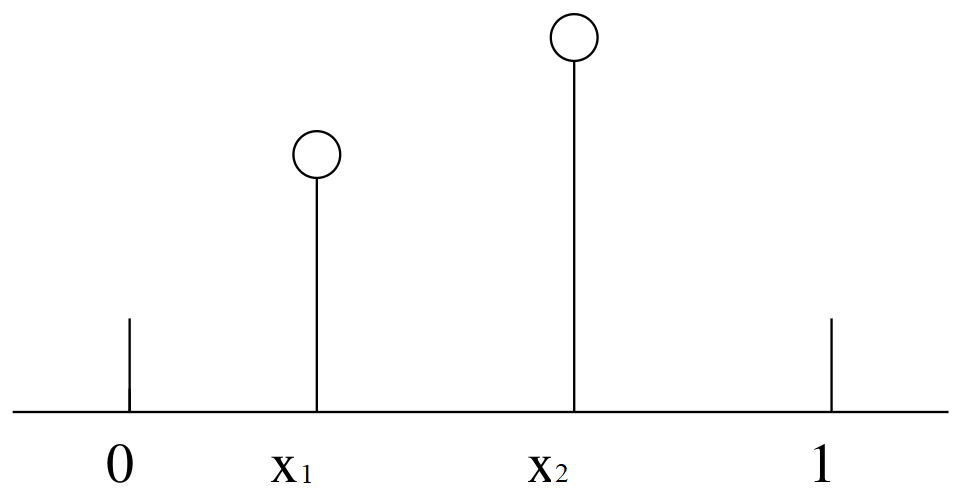
\includegraphics[width=0.9\textwidth]{img/17/f_unimodalna}
    \\
    $F(x)$ - f. unimodalna
  \end{frame}

  \begin{frame}{Metoda złotego podziału \emph{(golden section search)}}
    \begin{block}{Definicja funkcji unimodalnej}
      Funkcję $f(x)$ nazywamy \emph{unimodalną} na przedziale
      $[a{,}b]$ jeżeli:
      \begin{enumerate}
        \item $\exists x^{*}\in [a{,}b] : f(x^{*}) = min_{x \in [a{,}b]}f(x)$
        \item $\forall x_{1}{,}x_{2} : a \leq x_{1} < x_{2} \leq b$ zachodzi:
        \begin{itemize}
          \item $x_{2} \leq x_{*} \Rightarrow f(x_{1}) > f(x_{2})$
          \item $x_{1} \geq x_{*} \Rightarrow f(x_{1}) < f(x_{2})$
        \end{itemize}
      \end{enumerate}
    \end{block}
    \begin{itemize}
      \item Minimum -- w [0,1]
      \item Na początek -- potrzebne 2 punkty:
      $F(x_1),F(x_2) : F(x_1) < F(x_2) \Rightarrow \text{min} F(x)\in [0{,}x_2]$
      \item w $[0{,}x_2]$ już jest punkt $x_1$ -- dla kolejnej
      redukcji $\to$ wyznaczenie $F(x)$ tylko w jednym punkcie.
    \end{itemize}

  \end{frame}

  \begin{frame}{Metoda złotego podziału \emph{(golden section search)}}
    Rozmieczenie punktów:\\
    $t$ -- współczynnik redukcji po każdym etapie\\
    \centering
    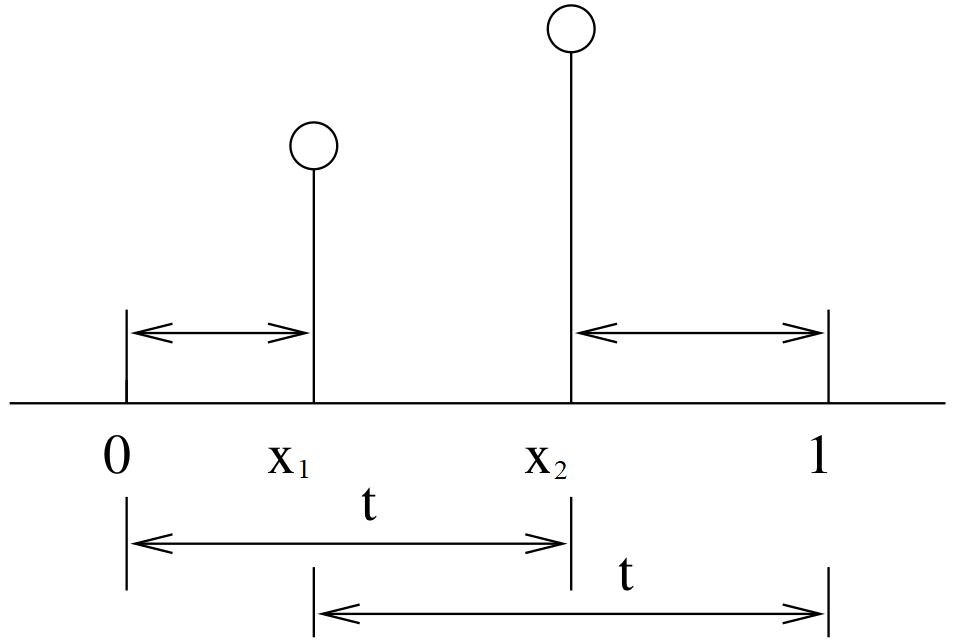
\includegraphics[height=0.6\textheight]{img/17/f_uni2}
  \end{frame}

  \begin{frame}{Metoda złotego podziału \emph{(golden section search)}}
    Po wyznaczeniu $F(x_3) \to$ długość przedziału : $t^{2}$
    \begin{displaymath}
      t^{2} = 1 - t \Rightarrow t = \frac{\sqrt{5} - 1}{2} \approx 0,616 \to \text{złoty podział}
    \end{displaymath}
    Dla zadanej ilości kroków -- optymalna $\to$ \emph{metoda Fibonacciego}\\
    $t$ -- zmienne, (1202 króliki)\\
    \centering
    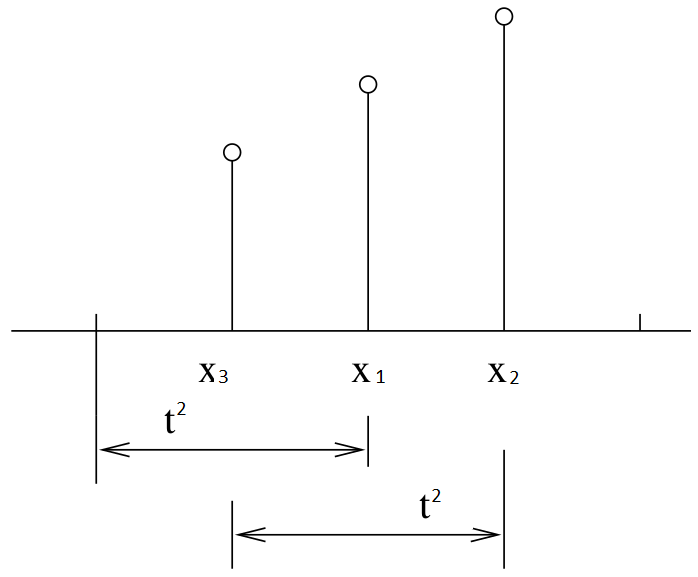
\includegraphics[height=0.55\textheight]{img/17/fibb}
  \end{frame}

  \begin{frame}{Metoda złotego podziału \emph{(golden section search)}}
    \begin{block}{Optymalność}
      W sensie minimax: minimalizuje maksymalną liczbę określen
      $F(x)$
    \end{block}
    \begin{block}{Optymalność pesymistyczna}
      Odpowiednik najleprzej strategii w grze przeciwko
      inteligentnemu przeciwnikowi.\\
      Podejście dobre dla patologicznych funkcjii.
    \end{block}
    \begin{block}{Metoda Bermana}
      $x_{0} = \frac{a + b}{2}$; poszukiwanie tam, gdzie maleje
      $\Rightarrow$ ustalony krok, w drugą stronę -- z mniejszym krokiem.
    \end{block}
  \end{frame}

\subsection{Kwadratowa interpolacja i aproksymacja}
  \begin{frame}{Kwadratowa interpolacja i aproksymacja}
    \begin{block}{Założenie: $F(x)$ jest parabolą}
      \begin{itemize}
        \item wyznaczamy $F(x)$ w 3 punktach: $x_{1}{,}x_{2}{,}x_{3}$
        (interpolacja f.~kwadr.)
        \item min $F(x) \to$ min paraboli przechodzącej przez
        $x_{1}{,}x_{2}{,}x_{3}$ znajduje się w punkcie $x_4$:
        \begin{displaymath}
          x_4 = \frac{
            \frac{F_{1}*(x_{2}+x_{3})}{(x_{1}-x_{2})*(x_{1}-x{3})} +
            \frac{F_{2}*(x_{1}+x_{3})}{(x_{2}-x_{1})*(x_{2}-x{3})} +
            \frac{F_{3}*(x_{1}+x_{2})}{(x_{3}-x_{1})*(x_{3}-x{2})}
          }{2 * [
            \frac{F_{1}}{(x_{1}-x_{2})*(x_{1}-x{3})} +
            \frac{F_{2}}{(x_{2}-x_{1})*(x_{2}-x{3})} +
            \frac{F_{3}}{(x_{3}-x_{1})*(x_{3}-x{2})}
          ]}
        \end{displaymath}
      \end{itemize}

    \end{block}
  \end{frame}

	%%%%%%%%%%%%%%%%%%%%%%%
	\section{Metody krokowe dla n-D (stepping methods in many variables)}

\subsection{Przeszukiwanie losowe}
  \begin{frame}{Przeszukiwanie losowe}

    \begin{block}{}
      \textbf{Problem: } Grid search na n-D -- złożoność czasowa $O(k^n)$.\\
      Algorytm niepraktyczny dla $n > 2$.\\
      \textbf{Rozwiązanie: } Metody Monte-Carlo -- Wybór próbek losowo.
    \end{block}

    \begin{block}{Realizacja}
   	  \begin{itemize}
   	  	\item[--] $\vec{x_i}$ - ustalane losowo, zgodnie z rozkładem:
   	  	\begin{itemize}
   		  \item równomiernym,
   		  \item normalnym
   	  	\end{itemize}
   	  	\item[--] Wybranie nalepszego znalezionego punktu.
   	  \end{itemize}
 	  \end{block}

    \begin{block}{}
      Stosowane, gdy:
      \begin{itemize}
        \item nic nie wiadomo o $F(x)$.
        \item $F(x)$ ma kilka minimów.
        \item dla ustalenia rozsądnego punktu startowego innych metod.
      \end{itemize}
    \end{block}
  \end{frame}

\subsection{Zmiana jednego parametru (Powell Search Method)}

  \begin{frame}{Zmiana jednego parametru}
    \begin{block}{Założenie}
      Funkcja $f$ -- ciągła na poszukiwanym obszarze.
    \end{block}
    \begin{block}{Obserwacja}
        Warunek na istnienie minimum - $ x_i $ -- \emph{stacjonarny punkt},
        tj. znikają wszystkie $n$ pochodne cząstkowe, $ \frac{\partial f}{\partial x_i} = 0 $ , $ i = 1,2,3,\ldots ,n $
    \end{block}
    \begin{block}{Powell Search Method}
        \begin{enumerate}
          \item Wybierz jeden z $n$ wymiarów.
          \item Wykonaj optymalizację 1-D na wybranym wymiarze.
          \item Powtarzaj do uzyskania punktu $x_i$, będącego minimum dla wszystkich wymiarów $n$.
        \end{enumerate}
    \end{block}
  \end{frame}

  \begin{frame}{Zmiana jednego parametru cd.}
    Przykład dwuwymiarowy.
	\begin{figure}
		\centering
		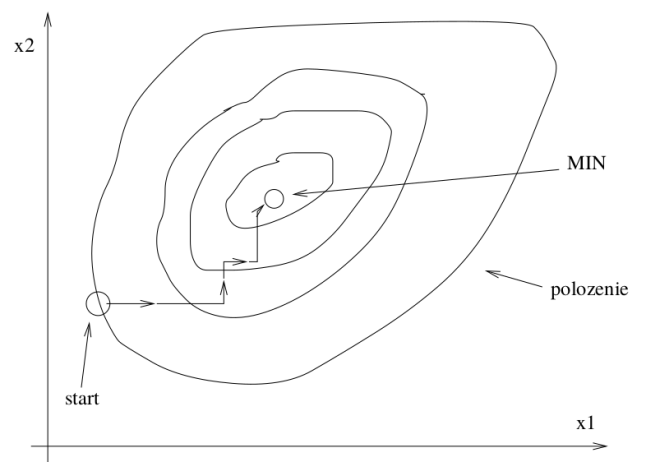
\includegraphics[height=0.6\textheight ,width=0.8\textwidth]{img/17/change_param_1}
	\end{figure}

  \end{frame}

  \begin{frame}{Zmiana jednego parametru cd.}

	Bardzo wolna z uwagi na przypadki z wąwozem (narrow valley):
	\begin{figure}
		\centering
		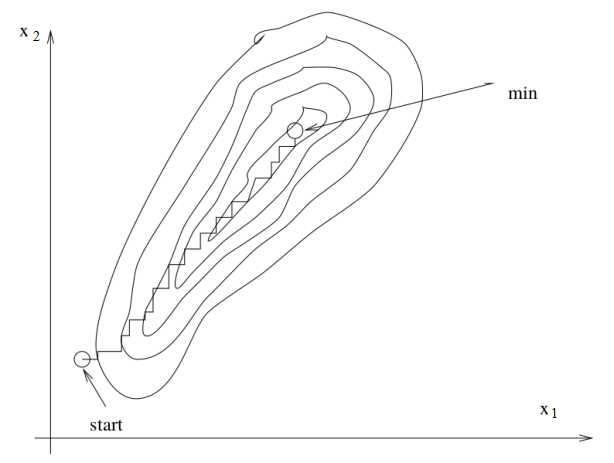
\includegraphics[height=0.6\textheight ,width=0.8\textwidth]{img/17/change_param_2}
	\end{figure}
	Dla takiego przykładu stosujemy ulepszone metody.

  \end{frame}

\subsection{Metoda Rosenbrocka}

  \begin{frame}{Metoda Rosenbrocka}

    \begin{block}{Algorytm}
 	  \begin{itemize}
   		\item Wykonaj jeden pełny cykl minimalizacji wzgl. kolejno wszystkich parametrów (współrzędnych),
   		\item Zmień osie układu współrzędnych - nowy układ ortogonalny:
   		\\jedna z osi od punktu początkowego do końcowego
   		\\w ostatnim cyklu minimalizacji,
   		\item Wykonaj kolejny cykl w nowym układzie współrzędnych.
  	\end{itemize}
  	\end{block}
  	  Metoda mało efektywna dla dużego $n$
  	  \\(w połączeniu z metodą aproks. kwadratowej.)

  \end{frame}

\subsection{Metoda simpleksów}

  \begin{frame}{Simplex - wprowadzenie}

    \begin{block}{Definicja}
 	  \textbf{Simplex} - najprostsza $n$-wymiarowa figura określona przez $(n+1)$ wierzchołków (vertex).
  	\end{block}
  	\begin{figure}
		\centering
		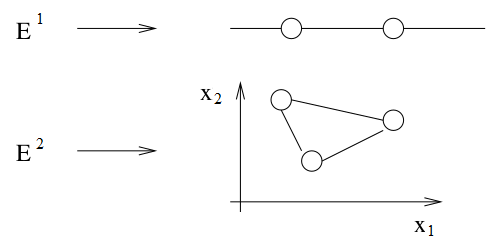
\includegraphics[height=0.3\textheight ,width=0.5\textwidth]{img/17/simplex}
	\end{figure}
  	\begin{block}{}
 	  \textbf{Nazwa metody} - w każdym kroku informacja o funkcji dotyczącej jej wartości w $n+1$ punktach
  	\end{block}

  \end{frame}

  \begin{frame}{Opis metody cz.1}

  	\begin{figure}
		\centering
		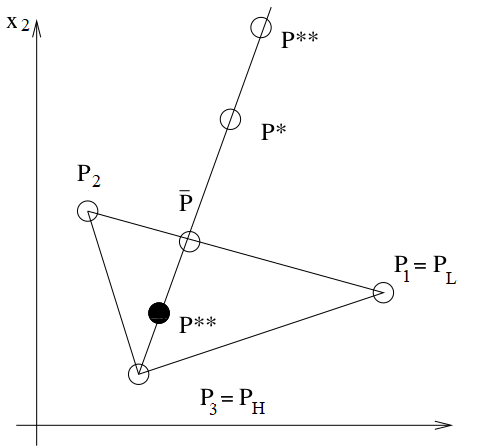
\includegraphics[height=0.8\textheight ,width=0.8\textwidth]{img/17/simplex_method}
	\end{figure}

  \end{frame}

  \begin{frame}{Opis metody cz.2}

	\begin{enumerate}
		\item Wybieramy (losowo, min 1-D) 3 punkty $P_1,P_2,P_3$
		\\i wyznaczamy spośród nich:
		\\ $P_H$ - gdzie $F$ największa (highest)
		\\ $P_L$ - gdzie $F$ najmniejsza (lowest)
		\item Wyznaczamy "środek masy" wszystkich punktów
		\\z pominięciem $P_H$
		  \begin{displaymath}
		    \overline{P}=\frac{1}{n}\left[\sum_{i=1}^{n+1}P_i-P_H\right]
		  \end{displaymath}
		\item Obliczamy odbicie $P_H$ wzgl. $\overline{P} : P$* $= \overline{P}+(\overline{P}-P_H)$ jeżeli
		\\ $F(P$*$) < F(P_L) \Rightarrow$ nowy $P$** $= \overline{P}+2*(\overline{P}-P_H)$
		\\ $F(P$*$) > F(P_L) \Rightarrow$ nowy $P$** $= \overline{P}-1/2*(\overline{P}-P_H)$
		\newcounter{saveenumi}	% do kontynuacji numeracji na następnym slajdzie
		\setcounter{saveenumi}{\value{enumi}}
	\end{enumerate}

  \end{frame}

  \begin{frame}{Opis metody cz.3}

	\begin{enumerate}
		\setcounter{enumi}{\value{saveenumi}}
		\item Punkt $P_H$ zastępujemy przez najlepszy z $P$* i $P$**
		\smallskip
		\\Jeżeli żaden z nowych punktów nie jest lepszy od $P_H$, tworzymy simplex oparty o $P_L$ w wymiarach $0.5$ $*$ poprzednie.
	\end{enumerate}
	Modyfikacje:
	\begin{itemize}
		\item Inne współczynniki $\neq 2$ oraz $\neq \frac{1}{2}$,
		\item Interpolacja kwadratowa wzdłuż prostej $(P_H,\overline{P})$
	\end{itemize}
    \begin{alertblock}{Uwaga}
 	  	Nowy punkt nie może być zbyt blisko $\overline{P}$, bo to grozi redukcją\\ (bez powrotu) simpleksów w $n$ do hiperpłaszczyzny.
    \end{alertblock}
  \end{frame}

  \begin{frame}{Opis metody cz.4}

	\begin{block}{Zalety :}
	  	\begin{itemize}
	  		\item[--] nieczuła na płytkie minima
	  		\\(pochodzenia: zaokrąglenia, statystyka \ldots),
	  		\item[--] mała ilość obliczeń funkcji $F(X)$ w każdym kroku,
	  		\item[--] największe możliwe kroki,
	  		\item[--] rozsądny kierunek poszukiwań,
	  		\item[--] bezpieczna i szybka daleko od minimum,
	  		\item[--] daje estymaty błędów parametrów
	  	\end{itemize}
    \end{block}
    \begin{block}{Zbieżność}
	  	$\underbrace{EDM}_{ \text{estimated distance to minimum}} = F(P_H) - F(P_L) < \underbrace{EPSI}_{(\epsilon)}$
    \end{block}

  \end{frame}

\subsection{Metody gradientowe}

  \begin{frame}{Metody gradientowe}

 	Działają w oparciu o informacje o funkcji w małych obszarach
 	\\(używany gradient i ew. wyższe pochodne).
    \begin{block}{Wyznaczanie pochodnych}
 	   analitycznie -- kłopotliwe, więc numerycznie:
 	   \begin{displaymath}
 	   	  \frac{\partial (F)}{\partial (x)} \bigg\vert_{x_0} \approx \frac{F(x_0+d) - F(x_0)}{d},
 	   	  \quad \delta \approx \frac{d}{2} \cdot \frac{\partial^2F}{\partial x^3}
 	   \end{displaymath}
 	   Lepiej:
 	   \begin{displaymath}
 	   	  \frac{\partial (F)}{\partial (x)} \bigg\vert_{x_0} \approx \frac{F(x_0+d) - F(x_0-d)}{2\cdot d},
 	   	  \quad \delta \approx \frac{d}{2} \cdot \frac{\partial^2F}{\partial x^3}
 	   \end{displaymath}
  	\end{block}

  \end{frame}

  \begin{frame}{Wyznaczanie pochodnych cd.}

    \begin{block}{}
      \begin{itemize}
 	      \item[--] $2 \cdot n$ wywołań $F(X)$ (symetryczne, gdy $2\ |\ n$)
 	      \item[--] Lecz łatwo przy okazji obliczyć drugie pochodne:
 	  	  \begin{displaymath}
 	   	  	\frac{\partial (F)}{\partial (x^2)} \bigg\vert_{x_0} \approx \frac{F(x_0+d) - 2 \cdot F(x_0) + F(x_0-d)}{d^2}
 	      \end{displaymath}
 	      Sprawdzić: drugie pochodne są stałe w małych obszarach - nie są potrzebne kroki symetryczne.
 	      \item[--] Drugie pochodne tworzą macierz $n \times n$.
      \end{itemize}
  	\end{block}

  \end{frame}

  \begin{frame}{Wyznaczanie pochodnych cd.}

    \begin{figure}
		\centering
		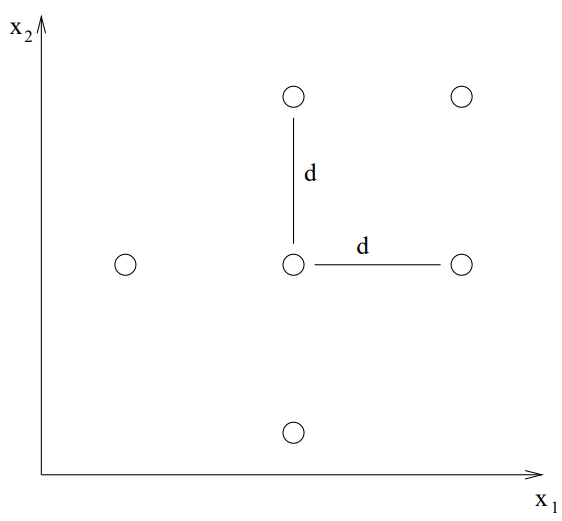
\includegraphics[height=0.6\textheight ,width=0.6\textwidth]{img/17/wyznaczanie_pochodnych}
	\end{figure}
    \begin{block}{}
      Poza p.~symetrycznymi potrzeba $\frac{n(n-1)}{2}$ pkt. (mieszane pochodne)
  	\end{block}

  \end{frame}

  \begin{frame}{Metody gradientowe}

    \begin{block}{Metoda największego spadku}
      Podążanie w kierunku wyznaczonym przez - $\vec g$ (gradient)
      \\(w tym kierunku funkcja maleje najszybciej) (Cauchy)
      \\$\left\{
        \begin{array}{l}
          \text{- seria minimalizacji 1-D wzdłuż kierunku największego spadku} \\
          \text{- iteracyjna, bo gradient nie jest stały}
	    \end{array}
	  \right.$
  	\end{block}
    \begin{figure}
		\centering
		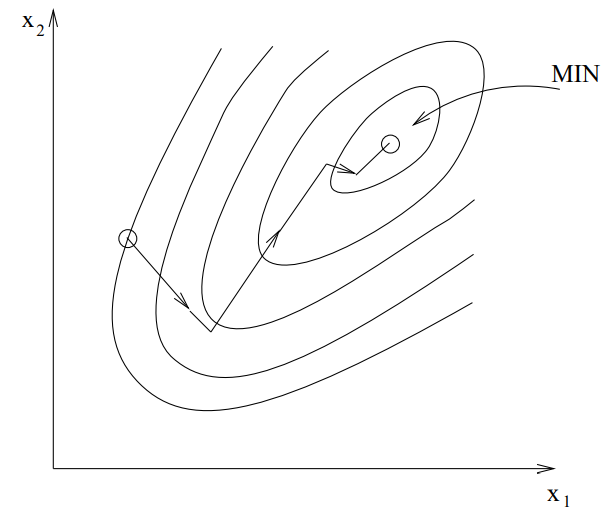
\includegraphics[height=0.5\textheight ,width=0.6\textwidth]{img/17/high_fall_met_1}
	\end{figure}

  \end{frame}

  \begin{frame}{Metoda największego spadku cd.}

    \begin{block}{}
      $\rightarrow$ Jeżeli minimalizacja w 1-D jest dokładna w kierunkach ortogonalnych -- \emph{met. uzmienniania 1 parametru}
      \smallskip
      \\Łatwo o przykład hipotetycznej funkcji,
      \\ dla której minimum jest $\perp$ gradientu.
  	\end{block}
    \begin{figure}
		\centering
		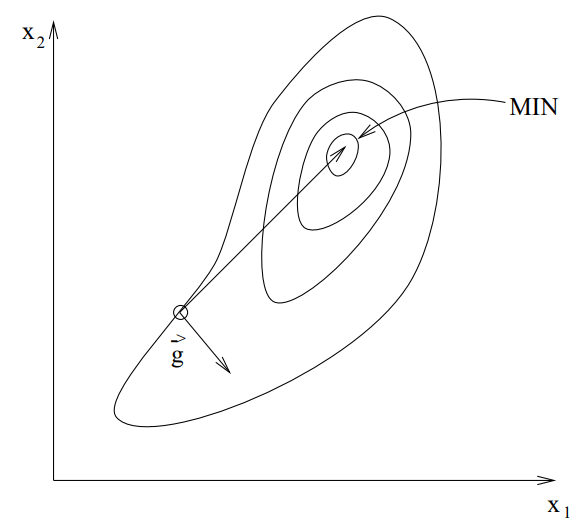
\includegraphics[height=0.5\textheight ,width=0.6\textwidth]{img/17/high_fall_met_2}
	\end{figure}

  \end{frame}

  \begin{frame}{Metody gradientowe}

    \begin{block}{Metoda Newtona}
      Ogólna funkcja kwadratowa jest określona przez:
      \\$\left.
        \begin{array}{l}
          \text{- wartość,} \\
          \text{- pierwsze pochodne} \\
          \text{- drugie pochodne}
	    \end{array}
	  \right\}$
	  $\begin{array}{l} \text{\emph{W dowolnym punkcie }} x_0 \\
     \text{Dysponujemy tymi informacjami} \end{array}$
	  \smallskip
	  \\Minimalizacja w pierwszym kroku.
	  \begin{displaymath}
	  		F(\vec{x}) = F(\vec{x_0}) + \vec{g}^T \cdot (\vec{x} - \vec{x_0}) +
	  		\frac{1}{2} (\vec{x} - \vec{x_0})^T \cdot G \cdot (\vec{x} - \vec{x_0})
	  \end{displaymath}
	  $\vec{g} - w \ \vec{x_0} \quad G$ -  stała macierz
	  \smallskip
	  \\Minimum:
	  \begin{displaymath}
	  		\vec{x_m} = \vec{x_0} - G^{-1} \cdot \vec{g} =  \vec{x_0} - V \cdot \vec{g}
	  \end{displaymath}
	\end{block}

  \end{frame}

  \begin{frame}{Metoda Newtona cd.}

    \begin{block}{}
      Sprawdzić: $V = G^{-1}$ -- macierz kowariancji (covariance)
      \\Jest to n-D odpowiednik 1-D interpolacji kwadratowej.
      \smallskip
	  \\ \emph{Te same wady!}
	  \begin{itemize}
	  	\item[--] niestabilna
	  	\item[--] rozbieżna, gdy $V$ nie jest dodatnio określona
	  \end{itemize}
	\end{block}
    \begin{block}{Zalety:}
      \begin{itemize}
	  	\item[--] krok nie jest dowolny, lecz określony przez metodę
	  	\item[--] kierunek $\neq$ wartość gradientu, tylko brana pod uwagę korelacja parametrów
	  \end{itemize}
	\end{block}

  \end{frame}

  \begin{frame}{Metoda Newtona cd.}

	\begin{block}{Używana:}
      \begin{itemize}
	  	\item[--] blisko minimum.
	  	\item[--] gdy funkcja jest dodatnio określoną formą kwadratową.
	  \end{itemize}
	\end{block}
	\begin{block}{}
	    Metoda Newtona jest podstawą wielu metod.
	\end{block}

  \end{frame}

  \begin{frame}{Metody gradientowe}

    \begin{block}{Dygresja: dodatnio określone formy kwadratowe}
      \emph{1-D forma kwadratowa:}
	  \begin{equation}
	  	F(x) = a + g \cdot x + \frac{1}{2} G \cdot x^2
      \nonumber
	  \end{equation}
    \begin{equation}
      g = \left.\frac{\partial F}{\partial x}\right|_{0}{,}\qquad
      G = \left.\frac{\partial^{2} F}{\partial x^2}\right|_{0}
      \nonumber
    \end{equation}
	  $F(x)$ ma min. wtedy i tylko wtedy, gdy $G$ $\geq 0$.
    \begin{equation}
	  		G = 0 \rightarrow \text{\emph{min}} \rightarrow \infty; \qquad
        x^m = -g/G
        \nonumber
	  \end{equation}
	  \emph{Dla ogólnej funkcji nieliniowej:}
	  \smallskip
	  \begin{itemize}
	  	    \item krok do $x = \frac{g}{G}$ gdy $G > 0$
	  	    \\(w przeciwnym przypadku: $\infty$ lub maximum)
	  \end{itemize}
	\end{block}

  \end{frame}

  \begin{frame}{Dodatnio określone formy kwadratowe cd.}

    \begin{figure}
		\centering
		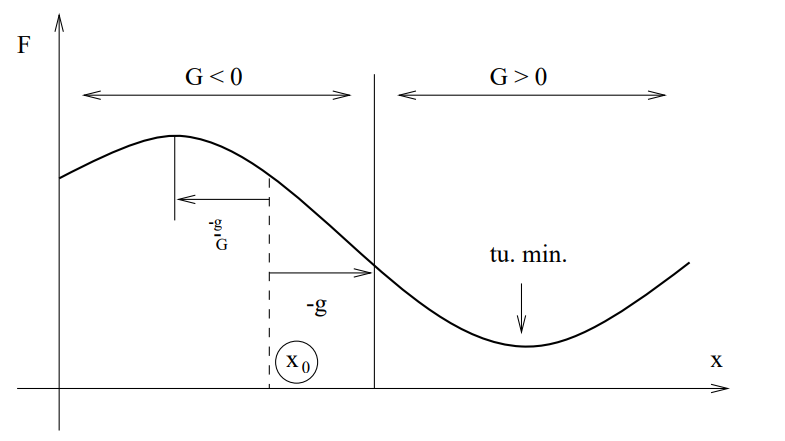
\includegraphics[width=0.95\textwidth]{img/17/dygresja}
	\end{figure}

  \end{frame}

  \begin{frame}{Dodatnio określone formy kwadratowe cd.}

    \begin{block}{}
    	\begin{itemize}
	  	    \item gdy $G \leq 0$ krok $= -g$
	  	    \\$\rightarrow$ kierunek - dobry,
	  	    \\$\rightarrow$ wartość - dowolna
	    \end{itemize}
	    W $x_0 \rightarrow F(x)$ nie jest wypukła (dodatnio określona)
	    \medskip\\
	    \emph{Uogólnienie na n-D:}\\
	    $g \rightarrow \vec{g}$, $G$ - macierz 2-ich poch.;
	    $F(\vec X) = a + \vec{g}^T \cdot \vec{x} + \frac{1}{2} \vec{x}^T G$ tylko dla $G$ dod. określonej
	    ma sens krok do:
	    \begin{displaymath}
	  		\vec{x} = - G^{-1} \cdot \vec{g}
	    \end{displaymath}
    \end{block}

  \end{frame}

  \begin{frame}{Metody gradientowe}

    \begin{alertblock}{}
      \textbf{Badanie czy $G$ jest dodatnio określona.}\\
      Brak prostych sposobów.
    \end{alertblock}
    \begin{block}{\emph{Dla macierzy kwadratowych, symetrycznych - 2 warunki konieczne}}
      $1^o$ elementy diagonalne $> 0$ \ (wyst. 1 $\times$ 1)
      \\$2^o$ elementy pozadiagonalne:
      \begin{displaymath}
      		G_{ij}^2 < G_{ii} \cdot G_{jj}
      \end{displaymath}
    \end{block}

  \end{frame}

  \begin{frame}{Badanie czy $G$ jest dodatnio określona cd.}

    \begin{block}{Ogólne warunki konieczne i wystarczające}
      \begin{itemize}
      		\item[--] wszystkie wartości własne $> 0$ (b. trudne i przybliżone)
      		\item[--] wyznacznik wszystkich macierzy $> 0$
      		\begin{figure}
				\centering
				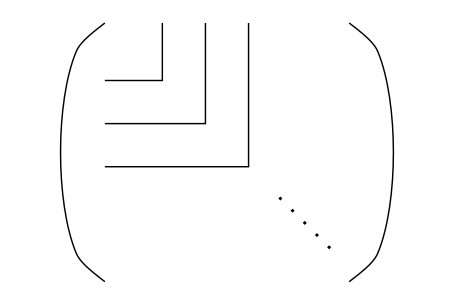
\includegraphics[height=0.2\textheight ,width=0.3\textwidth]{img/17/matrix}
			\end{figure}
			(najprościej sprawdzić)
			\item[--] skalar $E^T \cdot G\vec{e} > 0$ dla $\bigwedge \vec{e}$ (zwykłe $\rightarrow$ def.), wyjaśnia dlaczego $G$ dod.
			okr. daje formę $F(x)$ z minimum: $F(x)$ rośnie we wszystkich kierunkach od $\vec{e} = 0$
			\item[--] $-V = G^{-1}$ jest dodatnio określona
      \end{itemize}
    \end{block}

  \end{frame}

  \begin{frame}{Metody gradientowe}

 	\begin{block}{Postępowanie w przypadku $G$ - nie jest dod. określone}
 	   \begin{enumerate}[a)]
 	   		\item analogicznie do 1-D : G = I $\rightarrow$ Ale:
 	   		\item lepiej:
 	   		\begin{itemize}
 	   			\item[--] gdy $\bigwedge$ elementy diagonalne $G > 0$, wtedy pozadiag. $\rightarrow = 0$ (scale - invariant step),
 	   			\item[--] gdy tylko niektóre el. pozadiag. $G_{ij}^2 \geq G_{ii}G_{jj} \Rightarrow G_{ij} = 0$,
 	   			\item[--] zamiast $G^{-1}$ bierzemy $(G + \lambda \cdot I)^{-1}$;
 	   			\\ $\lambda \geq$ największa (bezwzgl.) ujemna wartość własna:
 	   			\begin{itemize}
 	   				\item[--] dużo obliczeń,
 	   				\item[--] krok pośredni pomiędzy m. Newtona a największego spadku
 	   				\\(duże $\lambda$ : krok krótki, w kierunku $\vec{g}$)
 	   			\end{itemize}
 	   			\item[--] gdy jedna lub więcej diagonalnych 2-ich poch. $< 0$
 	   			\\ $\Rightarrow$ informacja o kierunku wzrostu ujemnej 1-szej poch.
 	   			\\w tym kierunku - szukanie met. zmiany 1 param.
 	   		\end{itemize}
 	   \end{enumerate}
 	\end{block}

  \end{frame}

  \begin{frame}{Gdy $G$ - nie jest dodatnio określone cd.}

 	\begin{block}{}
 	Metody oparte na powyższych regułach - \emph{quasi-Newton method}
 	\medskip
 	\\Podstawowa wada tych metod - obliczanie i odwracanie
 	\\w każdym kroku macierzy drugich pochodnych
 	\smallskip
 	   	\begin{itemize}
 	   		\item[--] obliczanie 2-ich poch. $\sim n^2$ (długie)
 	   		\item[--] odwracanie
 	   	\end{itemize}
 	\end{block}

  \end{frame}

  \begin{frame}{Metody gradientowe}

 	\begin{block}{Metoda sprzężonych kierunków \emph{conjugate directions}}
 	   Wektory $\vec{d_i}$ i $\vec{d_j}$ \emph{są sprzężone} ze względu na dodatnio określoną macierz, jeżeli:
 	   \\$\vec{d_i}^T A\vec{d_j} = 0$ dla $i \neq j$;
 	   \\gdy $A = I, \vec{d_i} \rightarrow$ ortogonalne
 	   \\(sprzężenie - uogólnienie ortogonalności)
 	   \\ \textbf{n sprzężonych wektorów rozpina n-D przestrzeń}.
 	   \\$A$ - nie określa jednoznacznie zbioru wektorów sprzężonych $\rightarrow$ można zastosować
 	   \emph{uogólnienie procedury ortogonalizacji Grama-Schmidta}:
 	   \\$d_1$ - dowolny wektor $d_2 = A \cdot d_1 - \frac{d_1^T A A d_1}{d_1^T A d_1} \cdot d_1 \rightarrow$ sprzężony do $d_1$
 	   \\$d_3 =$ \ldots
 	   \begin{flushright}
 	      Zadanie: sprawdzić.
 	   \end{flushright}
 	\end{block}

  \end{frame}

  \begin{frame}{Metoda sprzężonych kierunków cd.}

    W minimalizacji użyteczne są wektory sprzężone
    \\ze względu na \emph{hesjan} $G$.
 	\begin{block}{Twierdzenie}
 	   Sekwencja liniowych minimalizacji w każdym z $n$ sprzężonych kierunków minimalizuje ogólną funkcję kwadratową $n$ zmiennych.
 	\end{block}
 	\begin{block}{Dowód:}
 	   $\left\{
        \begin{array}{l l}
          \text{funkcja:} & F(\vec{x}) = F(\vec{0}) + \vec{g}^T \vec{x} + \frac{1}{2} x^T G \vec{x} \\
          \text{kierunki sprzężone:} & \vec{d_i} \ \vec{d_i}^T G \vec{d_j} = 0 \ i \neq j
	    \end{array}
	  \right.$
	  \\gdzie: $G$ jest macierzą.
 	\end{block}

  \end{frame}

  \begin{frame}{Metoda sprzężonych kierunków cd.}

 	\begin{block}{Dowód cd.}
		\emph{$x, g$ -  jako kombinacje liniowe:} w układzie o wektorach jednostkowych
		\begin{displaymath}
			\vec{x} = \sum_i y_i \vec{d_i}, \quad \vec{g} = \sum_i c_i \vec{d_i}
		\end{displaymath}
		wtedy:
		\begin{displaymath}
			F(x) = F(0) + (\sum_i c_i \vec{d_i}^T) \cdot (\sum_j y_j \vec{d_j}) +
			\underbrace{\frac{1}{2} (\sum_i y_i \vec{d_i}^T) \cdot G \cdot (\sum_j y_j \vec{d_j})}_{(\star)}
		\end{displaymath}
 	\end{block}

  \end{frame}

  \begin{frame}{Metoda sprzężonych kierunków cd.}

 	\begin{block}{Dowód cd.}
 		($\star$) wynik przegrupowania:
		\begin{itemize}
			\item podwójna suma
			\item $i \neq j \Rightarrow$ równe zero (warunek sprzężenia)
		\end{itemize}
		\begin{displaymath}
			F(x) = F(0) + \sum_i \sum_i c_i d_i^T d_j y_j + \frac{1}{2} \sum_j y_j^2 d_j^T G d_j =
		\end{displaymath}
		\begin{center}
		   	\begin{tabular}{|c|}
		   	\hline
				$F(0) + \sum_j (b_j y_j + b'_j y_j^2)$
			\\ \hline
			\end{tabular}
			\smallskip
			\\gdzie:
			\begin{tabular}{|c|}
		   	\hline
				$b_j = \sum_i c_i d_i^T d_j{,} \quad b'_j = \frac{1}{2} d_j^T G d_j$ - \underline{stałe}
			\\ \hline
			\end{tabular}
		\end{center}
		\emph{zamiast} $\vec{x}$ \emph{- mamy} $\vec{y}$, przy czym $F(x)$ stała się \emph{sumą niezależnych jednoparametrowych} funkcji kwadratowych. Minimalizacja ze względu na $y_i$ (wzdłuż kierunku $\vec{d_i}$) jest niezależna od minimalizacji  względem pozostałych sprzężonych kierunków.
 	\end{block}

  \end{frame}

  \begin{frame}{Metoda sprzężonych kierunków cd.}

 	\begin{block}{Wnioski:}
		\begin{itemize}
			Minimalizacja nie wzdłuż osi ortogonalnych,
			\\ale wzdłuż kierunków sprzężonych
		\end{itemize}
 	\end{block}
 	\begin{block}{}
		Ale można szukać innej konstrukcji $d_i$ \emph{(gdy znamy $G$ - m. Newtona
		\\- w 1 kroku!)} $\Rightarrow$ \emph{Można wyznaczyć $d_i$ bez $G$!}
 	\end{block}
 	\begin{block}{Twierdzenie}
		Jeżeli $\vec{x_0}, \vec{x_1}$ - punkty min. w 2 równoległych podprzestrzeniach,
		\\to $(\vec{x_1} - \vec{x_0})$ jest sprzężony do każdego wektora w tych dwóch podprzestrzeniach.
 	\end{block}

  \end{frame}

  \begin{frame}{Metoda sprzężonych kierunków cd. }

 	\begin{block}{Dowód}
	  $\vec{x_0}$ - min. wzdłuż $d_i$; to gradient F w $\vec{x_0}$ musi być $\perp \vec{d_1}$
	  \smallskip
	  \begin{center}
	    $ \left\{
          \begin{array}{l}
            \vec{d_1}^T \cdot (\vec{g} + G \vec{x_0}) = 0 \\
            \vec{d_1}^T \cdot (\vec{g} + G \vec{x_1}) = 0
	      \end{array}
	    \right\} $
	    \ $(\vec{g}$ \emph{grad. w} $x = 0)$
	  \end{center}
	  \begin{center}
	    $\vec{d_1}^T \cdot G (\vec{x_1} - \vec{x_0}) = 0 \qquad (\vec{x_1} - \vec{x_0})$ sprzężony do $\vec{d_1}$
	  \end{center}
 	\end{block}

  \end{frame}

  \begin{frame}{Metoda sprzężonych kierunków cd. }

   \begin{block}{Dowód cd.}
	  W przestrzeni:
	  \smallskip
	  \\3-D $\Rightarrow$ 3 dodatkowe minimalizacje
	  \\ \ (3-ci kier. sprzężenia do 2 pierwszych)
	  \\n-D $\Rightarrow$ $\frac{n(n+1)}{2}$ minimalizacje - ile elem. w $G$ - ale:
	  \\ \ metoda bardzo stabilna dla $F(x) \neq$ kwadratowych i nie wymaga
	  \\ \ znajomości pochodnych
	  \medskip
	  \\Uwaga: \emph{asymetria:}
	  \begin{itemize}
	  	  \item $n$ minimal. w $d_1$
	  	  \item $1$ minimal. w $d_n$
	  \end{itemize}
 	\end{block}

  \end{frame}

  \begin{frame}{Metody gradientowe}

 	\begin{block}{Metoda gradientów sprzężonych \emph{(conjugate gradients)}}
 	   Wykorzystuje tylko 1-sze pochodne.
 	   \medskip
 	   \\ $F(\vec{x})$ i $\vec{g}(\vec{x})$ wyznaczone w $\vec{x_0}$ i $\vec{x_1}$, z nich:
 	   \smallskip
 	   \\ $\vec{\Delta x} = \vec{x_1} - \vec{x_0}$, \ $\vec{\Delta g} = \vec{g_1} - \vec{g_0}$
 	   \smallskip
 	   \\ Dla $F(\vec{x})$ kwadratowej, z hesjanem $G$:
 	   $\begin{array}{|c|}
 	   	  \hline
 	   	  \vec{\Delta g} = G \cdot \vec{\Delta x}
 	   	  \\ \hline
 	   \end{array}$,
 	   \\zatem dowolny $\vec{d_1} \perp \vec{\Delta g}$ będzie dodany do $\vec{\Delta x}$:
 	   \begin{center}
 	      $\begin{array}{|c|}
 	   	    \hline
 	   	    \vec{d_1}^T \cdot \vec{\Delta g} = \vec{d_1} G \vec{\Delta x} = 0
 	   	    \\ \hline
 	      \end{array}$
 	   \end{center}
 	   \smallskip
 	   Metoda uzyskiwania kierunków sprzężonych \emph{bez} znajomości $G$:
 	   \\Pierwszy kierunek: $\vec{d_0} = \vec{-g_0}$
 	   \\min. wzdłuż $\vec{d_0}$ : w $\vec{x_1}$, gradient:  $\vec{g_1}$
 	   \\Drugi kierunek: $\vec{d_1} = -\vec{g_1} + b \cdot \vec{d_0}$
 	   \\(liniowa kombinacja znanych kierunków)
 	\end{block}

  \end{frame}

  \begin{frame}{Metoda gradientów sprzężonych cd. }

   \begin{block}{}
	  Warunek sprzężenia: $\vec{d_1}^T \cdot G \cdot \vec{d_0} = \vec{d_1}^T \cdot G \cdot (\vec{g_1} - \vec{g_0}) = 0$, czyli:
	  $(-\vec{g_1} + b \cdot \vec{d_0}) \cdot G \cdot \vec{d_0} = (-\vec{g_1} -b \cdot \vec{g_0}) \cdot (\vec{g_1} - \vec{g_0}) = 0$
	  \\$\vec{x_1}$ - to min. wzdłuż $\vec{d_0} = -\vec{g_0} \Rightarrow \vec{g_0} \perp \vec{g_1} : \vec{g_1}^T \cdot \vec{g_0} = 0$
	  \smallskip
	  \\$\Rightarrow$
	  $\begin{array}{|c|}
 	   	 \hline
 	   	    b = \frac{\vec{g_1}^T \cdot \vec{g_1}}{\vec{g_0}^T \cdot \vec{g_0}}
 	   	 \\ \hline
	  \end{array}$,
 	  czyli nowy sprzężony kierunek $\vec{d_1} = -\vec{g_1} + \left(\frac{\vec{g_1}^T \cdot \vec{g_1}}{\vec{g_0}^T \cdot \vec{g_0}}\right) \cdot \vec{d_0} $
 	  \medskip
 	  \\Ten proces kontynuujemy generując $n$ kierunków \\ wzajemnie sprzężonych.
 	  \medskip
 	  \\Można pokazać, że dla wszystkich sprzężonych kierunków zachodzi:
 	  \begin{center}
 	  	 $\begin{array}{|c|}
 	   	   \hline
 	   	      \vec{d_{i+1}} = -\vec{g_{i+1}} + \frac{\vec{g_{i+1}}^T \cdot \vec{g_{i+1}}}{\vec{g_{i}}^T \cdot \vec{g_{i}}} \cdot \vec{d_i}
 	   	   \\ \hline
	    \end{array}$
 	  \end{center}
 	\end{block}

  \end{frame}

	%%%%%%%%%%%%%%%%%%%%%%%
	\section{Metoda zmiennej metryki}

\subsection{Metoda Newtona -- podsumowanie}
  \begin{frame}
    \begin{block}{Uogólniona met. Newtona -- znajdowanie minimum}
      \textbf{Założenia: } Dana jest funkcja $F$, taka że $F(x) \in \mathbb{C}^2$.
    \end{block}
    \begin{block}{Procedura iteracyjna}
      W k-tym kroku:
      \begin{equation}\label{eq:def_0}
        \left.
          \begin{aligned}
            x_{k + 1} &= x_{k} + \alpha_{k} \cdot d_{k}\\
            d_{k}     &= - V(x_k) \cdot \nabla F(x_{k})\\
            V(x_k)    &= H^{-1}(x_{k})
          \end{aligned}
       \right\}
      \end{equation}
    \end{block}
  \end{frame}

  \begin{frame}{}
    \begin{block}{Oznaczenia}
      $d_{k}$ -- wektor kierunku poszukiwań\\
      $\alpha_{k}$ -- długość kroku; dobrana tak, aby\\
      \hspace*{8mm} minimalizować funkcję $\alpha \mapsto F(x_{k} + \alpha \cdot d_{k}), \alpha \geq 0$\\
      $H(x_k) = \bigg[ \frac{\partial^2 F(x_{k})}{\partial x_{i} x_{j}} \bigg]$ -- hesjan funkcji $F(x_{k})$\\
      $G(x_k)$ -- hesjan formy kwadratowej $Q$ w punkcie $x_k$\\
      \begin{equation*}
        Q(x) = (Ax - c)^T \cdot (Ax - c)
      \end{equation*}
      $V(x_k) = G^{-1}(x_k)$ -- macierz kowariancji w k-tym kroku
    \end{block}

    \begin{block}{}
      \textbf{Istota: } $V(x_{k})$ -- obliczane w każdym kroku.\\
      Duży narzut obliczeniowy.
    \end{block}
  \end{frame}

  \begin{frame}{Optymalizacja metodami zmiennej metryki}
    \begin{block}{}
      \textbf{Cel: } Zmniejszenie narzutu obliczeniowego na wyznaczanie $V_k$.\\
      \textbf{Pomysł: } Wykorzystanie informacji z poprzednich kroków iteracyjnych.
    \end{block}

    \begin{block}{}
      \textbf{Szukamy: }
        \begin{equation}\label{eq:v_k_c}
          V_{k + 1} = V_k + C_k
        \end{equation}
      \textbf{Dysponujemy: } $x_k, x_{k + 1}, \nabla F(x_k), \nabla F(x_{k + 1})$
    \end{block}
  \end{frame}

  \begin{frame}{Kierunki sprzężone}
    \begin{block}{Kierunki wzajemnie sprzężone}
      \textbf{Def: } Kierunki $d_0, d_1, ..., d_i, ..., d_r, d_i \neq 0, r \leq n - 1$\\
      nazywamy wzajemnie sprzężonymi względem macierzy\\
      $A$ (A-sprzężonymi), jeśli:
      \begin{equation*}
        d_i^T A d_j = 0, i \neq j
      \end{equation*}
      Jest to uogólnienie def. ortogonalności:
      \begin{equation*}
        V^T \cdot u = V^T \cdot I \cdot u = 0
      \end{equation*}
      Wektory własne $A$ symetrycznej są wektorami A-sprzężonymi.
    \end{block}
  \end{frame}

  \begin{frame}{Minimalizacja w kierunkach sprzężonych}
    \begin{block}{Twierdzenie o minimalizacji w kierunkach sprzężonych}
      \textbf{Założenie: } $d_0, d_1, .., d_{n - 1}$ -- ciąg wektorów A-sprzężonych\\
        A -- macierz $(n \times n)$, symetryczna, dodatnio określona.\\
      \textbf{Twierdzenie: } Niezależnie od wyboru punktu początkowego $x_0$\\
       można zminimalizować formę kwadratową:
       \begin{equation}\label{eq:tw_1}
         Q(x) = Q(x_0) + b^T \cdot x + \frac{1}{2} x^T \cdot A \cdot x
       \end{equation}
       \begin{enumerate}
         \item w najwyżej $n$ krokach iteracyjnych\\
         \item kolejne minimalizacje -- wzdłuż $d_i$\\
         \item każdy wektor $d_i$ -- używany tylko jeden raz\\
         \item kolejność wprowadzenia $d_i$ do obliczeń -- obojętna
       \end{enumerate}
    \end{block}
  \end{frame}

  \begin{frame}{Minimalizacja w kierunkach sprzężonych -- dowód}
    $V$ -- dowolny wektor; $d_i$ -- liniowo niezależne
    \begin{equation}
      \begin{gathered}
        \begin{aligned}
          &V = \sum_{i=0}^{n - 1} \gamma_i \cdot d_i, &\gamma_i = \frac{d_i A v}{d_i^T A d_i}
        \end{aligned}
      \end{gathered}
    \end{equation}
    W kroku iteracyjnym $p$:
    \begin{equation*}
        \begin{aligned}
          &x_p = x_0 + \sum_{i = 0}^{p - 1} \alpha_i \cdot d_i, &p > 1
        \end{aligned}
    \end{equation*}
    $x_p$ -- kolejny punkt uzyskany w trakcie minimalizacji\\
    formy kw. $Q(x)$ wzdłuż kierunków $d_0, d_1, ..., d_{p - 1}$.
  \end{frame}

  \begin{frame}{Minimalizacja w kierunkach sprzężonych -- dowód cd.}
    \begin{enumerate}
      \item Z punktu $x_p$ do $x_{p + 1}$ przechodzimy wzdłuż $d_p$
      \item Forma $Q$ ma mieć minimum wzdłuż $d_p$
    \end{enumerate}
    Otrzymujemy więc, że:
    \begin{equation}\label{eq:d_n_q_zero}
        \begin{aligned}
          d_p^T \nabla Q(x_{p + 1}) = 0
        \end{aligned}
    \end{equation}
    Po podstawieniu $(\ref{eq:tw_1})$ do $(\ref{eq:d_n_q_zero})$:
    \begin{equation*}
        \begin{aligned}
          d_p^T \cdot A \cdot \bigg[(x_0 + \sum_{i = 0}^{p - 1} \alpha_i \cdot d_i) + \alpha_p \cdot d_p \bigg] + d_p^T \cdot b = 0
        \end{aligned}
    \end{equation*}
    Z czego wyznaczamy stałą:
    \begin{equation*}
        \begin{aligned}
          \alpha_p = - \frac{d_p^T (A \cdot x_0 + b)}{d_p^T \cdot A \cdot d_p}
        \end{aligned}
    \end{equation*}
  \end{frame}

  \begin{frame}{Minimalizacja w kierunkach sprzężonych -- dowód cd.}
    W konsekwencji po co najwyżej $n$ krokach, (bo może być $\alpha_i = 0)$ zachodzi:
    \begin{equation*}
        \begin{aligned}
          x_n = x_0 - \sum_{i = 0}^{n - 1} \frac{d_i^T (A \cdot x_0 + b) d_i}{d_i^T \cdot A \cdot d_i} =
          x_0 - \underbrace{\sum_{i = 0}^{n - 1} \frac{d_i^T \cdot A (x_0 + A^{-1} b) d_i}{d_i^T \cdot A \cdot d_i}}_{x_0 + A^{-1} \cdot b}\\
          x_n = x_0 - x_0 - A^{-1} \cdot b = - A^{-1} \cdot b
        \end{aligned}
    \end{equation*}
    Osiągnęliśmy min. formy kwadratowej:
    \begin{enumerate}
      \item niezależnie od kolejności wystąpień $d_i$,
      \item w co najwyżej $n$ krokach minimalizacyjnych
    \end{enumerate}
    Met. kier. sprzężonych prowadzi do \textbf{zbieżności kwadratowej}.
  \end{frame}

  \begin{frame}{Minimalizacja w kierunkach sprzężonych 2}
    \begin{block}{Twierdzenie 2}
      \textbf{Założenie: } $x_{k + 1}$ -- kolejny punkt uzyskany w minimalizacji\\
      formy $(\ref{eq:tw_1})$ wzdłuż A-sprzężonych kierunków $d_0, d_1, ..., d_k$.\\
      \textbf{Twierdzenie: } Zachodzi równanie:
      \begin{equation}\label{eq:tw_2}
          \begin{aligned}
            &d_l^T \nabla Q(x_{k + 1}) = 0, &l = 0, 1, ..., k
          \end{aligned}
      \end{equation}
    \end{block}

    \begin{block}{}
        \textbf{Obserwacja: } Gradient formy kwadratowej w punkcie $x_p$ "pamięta"
        wszystkie poprzednie kierunki sprzężone\\ prowadzące do $x_p$ z $x_0$.
    \end{block}
  \end{frame}

  \begin{frame}{Minimalizacja w kierunkach sprzężonych 2 -- dowód}
    \begin{equation*}
      \begin{aligned}
        \nabla Q_{k + 1}  &= A \cdot x_{k + 1} + b = A \cdot \bigg(x_s + \sum_{j = s + 1}^k \alpha_j d_j \bigg) + b =\\
                          &= \nabla Q_{s + 1} + \sum_{j = s + 1}^{k} \alpha_j A d_j
      \end{aligned}
    \end{equation*}
    W konsekwencji:
    \begin{equation*}
      \begin{aligned}
        d_s^T \nabla Q_{s + 1} = \underbrace{d_s^T \nabla Q_{s + 1}}_{= 0 \text{ (wzór \ref{eq:d_n_q_zero})}}
        + \underbrace{\sum_{j = s + 1}^k \alpha_j d_s^T A d_j}_{= 0}
      \end{aligned}
    \end{equation*}
    Słuszne jest więc równanie $(\ref{eq:tw_2})$.
  \end{frame}

  \begin{frame}{Formuła Davidona-Fletchera-Powella}
      Dla macierzy $V = G^{-1}$:\\
      \begin{enumerate}
        \item $(n \times n)$\\
        \item symetrycznej\\
        \item dodatnio określonej
      \end{enumerate}
      wektorów $d_0, d_1, ..., d_{n - 1}$ wyznaczającej kierunki sprzężone wzgl. $G$\\
      zachodzi:
      \begin{equation}
        \begin{aligned}
          V = \sum_{i = 0}^{n - 1} \frac{d_i d_i^T}{d_i^T G d_i}
        \end{aligned}
      \end{equation}
  \end{frame}

  \begin{frame}{Formuła Davidona-Fletchera-Powella 2}
    Bierzemy element tej sumy jako pierwsze przybliżenie do szukanej
    poprawki $C_k$ (wzór $\ref{eq:v_k_c}$):
    \begin{equation}\label{eq:v_k1_k}
      \begin{aligned}
        &V_{k + 1} = V_k + \frac{d_k d_k^T}{d_k^T G d_k} + B_k, &B_k = B_k^T
      \end{aligned}
    \end{equation}
    $B_k$ -- z warunku: $d_0, d_1, ..., d_k$ -- kierunki G-sprzężone.
  \end{frame}


  \begin{frame}{Formuła Davidona-Fletchera-Powella 3}
    Przymując:
    \begin{equation*}
      \begin{aligned}
        V_k G d_i = d_i, i = 0, 1, ..., k
      \end{aligned}
    \end{equation*}
    dla $d_0, d_1, ..., d_k$ będących G-sprzężonymi.\\
    Mamy (wzór \ref{eq:def_0}):
    \begin{equation*}
      \begin{aligned}
        -d_i^T G d_{k + 1} &= d_i^T G V_{k + 1} \nabla Q(x_{k + 1}) =\\
        = \bigg[ \nabla^T Q_{k + 1} V_{k + 1} G d_i \bigg]^T
        &= d_i^T \nabla Q_{k + 1} = 0 \text{, } i = 0, 1, ..., k
      \end{aligned}
    \end{equation*}
    Jest to wzór $(\ref{eq:tw_2})$.\\
    Wniosek: $d_{k + 1}$ -- również sprzężony do poprzednich.
  \end{frame}

  \begin{frame}{Formuła Davidona-Fletchera-Powella 4}
    Żądamy, aby:
    \begin{equation*}
      \begin{aligned}
        &V_{k + 1} G d_i = d_i, &i = 0, 1, ..., k+1
      \end{aligned}
    \end{equation*}

    Podstawiamy $V_{k + 1}$ z równania $(\ref{eq:v_k1_k})$ dla $i = k$.
    Otrzymujemy:\\
    \begin{equation*}
      \begin{aligned}
        \bigg(V_k + \frac{d_k d_k^T}{d_k^T G d_k} + B_k \bigg) G d_k = d_k
      \end{aligned}
    \end{equation*}

    Po przekształceniu:\\
    \begin{equation*}
      \begin{aligned}
        (V_k + B_k) G d_k = 0
      \end{aligned}
    \end{equation*}

    Co po uwzgl. wzorów $(\ref{eq:d_n_q_zero})$ i $(\ref{eq:def_0})$ daje:\\
    \begin{equation}
      \begin{aligned}
        \big[ \nabla Q_{k + 1} - \nabla Q_k \big]^T (V_k + B_k) = 0
      \end{aligned}
    \end{equation}
  \end{frame}

  \begin{frame}{Formuła Davidona-Fletchera-Powella 5}
    $B_k$ powinna mieć postać:
    \begin{equation*}
      \begin{aligned}
        B_k = - \frac{V_k \gamma_k \gamma_k^T V_k}{\gamma_k^T V_k \gamma_k}
      \end{aligned}
    \end{equation*}
    \begin{equation}
      \begin{aligned}
        \gamma_k = \nabla Q(x_{k + 1}) - \nabla Q(x_k)
      \end{aligned}
    \end{equation}
    \begin{equation}
      \begin{aligned}
        \delta_k \equiv x_{k + 1} - x_k \stackrel{(\text{wzór } \ref{eq:def_0})}{=} -\alpha_k G^{-1} \nabla Q_k = \alpha_k d_k
      \end{aligned}
    \end{equation}
    Otrzymujemy:
    \begin{equation*}
      \begin{aligned}
        d_k^T G d_k = \frac{(\alpha_{k + 1} - x_k)^T}{\alpha_k} G d_k = \frac{\gamma_k^T d_k}{\alpha_k}
      \end{aligned}
    \end{equation*}
    Gdyż dla formy kwadratowej:
    \begin{equation}
      \begin{aligned}
        \delta_k = G^{-1} \gamma_k
      \end{aligned}
    \end{equation}
  \end{frame}

  \begin{frame}{Metoda zmiennej metryki}
    \begin{block}{Wzór korekcyjny}
        Wzór korekcyjny ma postać:
        \begin{equation*}
          \begin{aligned}
            V_{k + 1} = V_k + \frac{\delta_k \delta_k^T}{\gamma_k^T \delta_k} - \frac{V_k \gamma_k \gamma_k^T  V_k}{\gamma_k^T  V_k \gamma_k}
          \end{aligned}
        \end{equation*}
    \end{block}
  \end{frame}

  \begin{frame}{Metoda zmiennej metryki -- przykład}
    \begin{equation*}
      \begin{rcases}
        \text{Geometria różniczkowa} \\
        \text{Ogólna teoria wzgl.}
      \end{rcases}
      \text{ Własności F}
    \end{equation*}
    F -- nieeuklidesowa przestrzeni zmiennych $x=(x_1, x_2, ..., x_n)$.\\

    Podst. niezmiennik:
    \begin{equation*}
      \begin{aligned}
        &ds^2 = dx^T A dx &\text{(kwadrat elem. długości)}
      \end{aligned}
    \end{equation*}

    \begin{equation*}
      \begin{aligned}
        dx - \text{przesunięcie, } x &\rightarrow x + dx \\
        A &\rightarrow \text{kowariantny tensor metryczny}
      \end{aligned}
    \end{equation*}
    \begin{equation*}
      \begin{aligned}
        \text{Dla } Q &\rightarrow A - \text{wszędzie stałe}\\
                    F &\rightarrow \text{przestrzeń o zmiennej metryce}
      \end{aligned}
    \end{equation*}
  \end{frame}

	%%%%%%%%%%%%%%%%%%%%%%%
	\section{Przypadki specjalne}

\subsection{Liniowy model}
  \begin{frame}{Liniowy model}
    \begin{block}{Minimalizacja $\chi^{2}$ (chisquare minimization, least squares fitting)}
      \begin{displaymath}
        min!F(\vec{x}) = \sum_{k=1}^{k} \left[ \frac{Y_{k} - T_{k}(\vec{x})}{\sigma_{k}} \right]^{2} = \sum_{k=1}^{k} f_{k}^{2}(\vec{x})
      \end{displaymath}
      gdzie: $Y_{k}$ -- wartości zamierzone, $\sigma_{k}$ -- błąd,\\
      $T_{k}$ -- wartości teoretyczne; $k \geq n$, zwykle $k \gg n$ \\
      \begin{tabular}{|c|} \hline
        min$F(\vec{x})$ \\ \hline
      \end{tabular}
      $\Rightarrow$ najlepsze estymaty parametrów $\vec{x}$
      (modelu teoretycznego)
    \end{block}

  \end{frame}

  \begin{frame}{Liniowy model}
    \begin{displaymath}
      (*)\ \frac{\partial^2 F}{\partial x_{i} \partial x_{j}} =
      \frac{\partial}{\partial x_{i}} \frac{\partial}{\partial x_{j}}
      \sum_{k} f_{k}^2 = \frac{\partial}{\partial x_{i}}
      \sum_{k} 2 \cdot f_{k} \cdot \frac{\partial f_{k}}{\partial x_{j}} =
    \end{displaymath}
    % \begin{displaymath}
    %   \sum_{k} 2 \cdot \frac{\partial f_{k}}{\partial x_{i}} \cdot
    %   \frac{\partial f_{k}}{\partial x_{j}} +
    %   \sum_{k} 2 \cdot f_{k} \cdot
    %   \frac{\partial^2 f_{k}}{\partial x_{i} \partial x_{j}}
    %
    % \end{displaymath}
    $(**)$ - zwkle uznajemy tem człon za mały w porównaniu
    z poprzedniem\\
    $\Rightarrow$ \emph{linearyzacja} (modelu! $T_{k}(x)$ -- liniowe)
  \end{frame}

  \begin{frame}{Liniowy model}
    %needs further formatting
    \emph{gdy drugi człon w} $(*)$ = 0 $\Rightarrow$
    linear least squares $\to F(x)$ -- quadratic; \\
    i cały problem minimalizacji $\Rightarrow$ znalezienie
    macierzy $\left[ \frac{\partial^2 F}{\partial x_{i} \partial x_{j}} \right]^{-1}$
    a znalezienie min!$F(x)$ w pojedyńczym kroku newtonowskim;\\
    \emph{gdy drugi człon w} $(*) \approx 0 \Rightarrow$
    non-linear least squares\\
    \begin{itemize}
      \item $\frac{\partial^2 F}{\partial x_{i} \partial x_{j}}$
      łatwe do policzenia (positiv defined)
      \item kilka kroków $\to$ iteracyjnie
      \item macierz $\left[ \frac{\partial^2 F}{\partial x_{i} \partial x_{j}} \right]^{-1}$
      nie zbiega się do macięrzy kowariancji
    \end{itemize}
  \end{frame}

	%%%%%%%%%%%%%%%%%%%%%%%
	\section{Minimum lokalne i globalne}

\subsection{Wprowadzenie}

  \begin{frame}{Wprowadzenie}
    Predstawione powyżej metody działają przy założeniu:\\
    $F(x)$ -- \emph{unimodalna} (w badanym obszarze)
    \begin{block}{Zwykle $F(x)$ ma wiele minimów $\Rightarrow$ wtedy 4 możliwości:}
      \begin{enumerate}
        \item \emph{wystarca znajomość dowolnego minimum lokalnego}\\
        $\to$ rzadko; najprościej
        \item \emph{szukamy minimum globalnego}\\
        $\to$ najczęściej $\Rightarrow$ zwłaszcza w optymalizacji;\\
        brak ogólnych pewnych metod % TODO: underline "pewnych"

      \end{enumerate}
    \end{block}
  \end{frame}

  \begin{frame}{Wprowadzenie}
    \begin{block}{}
      \begin{enumerate}
        \setcounter{enumi}{2}
        \item \emph{interesuje nas jedno ("fizyczne") minimum
        (niekoniecznie) globalne}\\
        $\to$ w badaniach naukowych; z góry znana przybliżona
        lokalizacja minimum $\to$ "dobra dolina". \\
        Poszukiwanie: od ustalenia przybliżonych, przewidywanych
        wartości części parametrów, znalezienie minimum ze
        względu na wszyskie parametry.
        \item \emph{szukamy wszyskich lokalnych minimów
        (w tym globalnego)} \\
        $\to$ najtrudniej, brak ogólnej metody
      \end{enumerate}
    \end{block}
  \end{frame}

\subsection{Algorytm Gelfanda-Cetlina (stepping m.)}
  \begin{frame}{Algorytm Gelfanda-Cetlina (stepping m.)}
    \begin{center}
      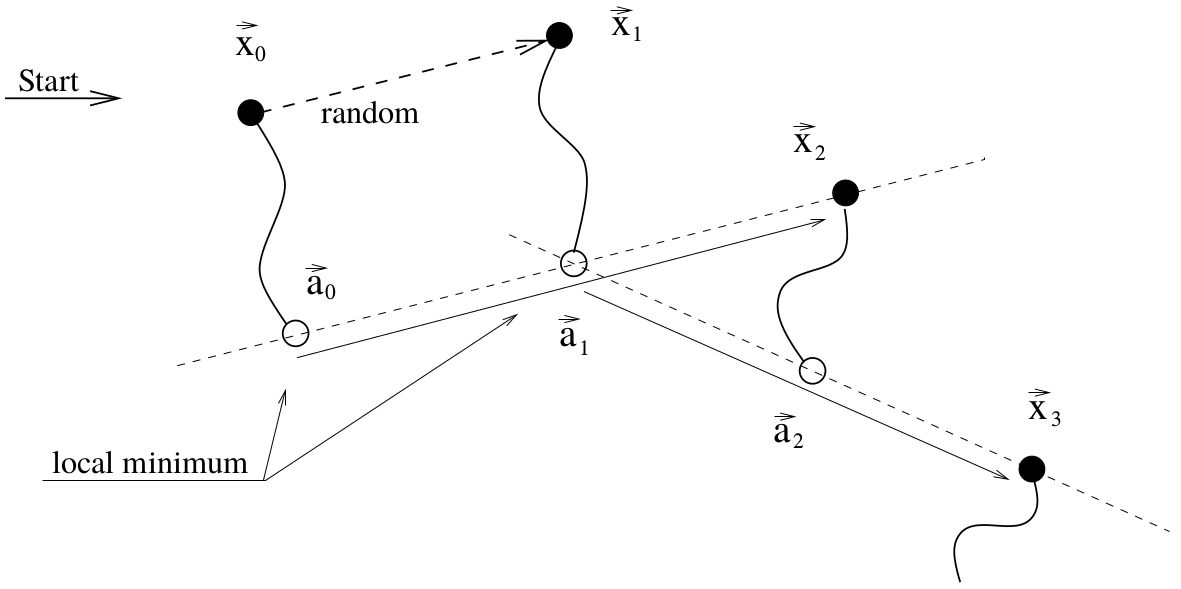
\includegraphics[width=1\textwidth]{img/17/algo_g-c}
    \end{center}
  \end{frame}

  \begin{frame}{Algorytm Gelfanda-Cetlina (stepping m.)}
    \begin{enumerate}
      \item z $\vec{x_{0}}$ -- lokalna minimalizacja $\Rightarrow$
      min. w $\vec{a_{0}}$
      \item z $\vec{x_{0}}$ -- długi, losowy krok do $\vec{x_{1}}$
      \item z $\vec{x_{1}}$ -- lokalna minimalizacja $\Rightarrow$
      min. w $\vec{a_{1}}$
      \item długi krok (precipitous step) wzdłuż
      $\vec{a_{1}} - \vec{a_{0}}$ do $\vec{x_{2}}$
      \item z $\vec{x_{2}}$ -- lokalna minimalizacja $\Rightarrow$
      min. w $\vec{a_{2}}$
      \item długi krok wzdłuż $\vec{a_{2}} - \vec{a_{1}}$ \dots itd.
    \end{enumerate}
  \end{frame}

  \begin{frame}{Algorytm Gelfanda-Cetlina (stepping m.)}
    \begin{block}{Metoda jest nielokalna}
      Przeszukiwanie zarówno w kierunku rosnących jak i
      malejących wartości $F(x)$, z preferencją w kierunku
      malejących (przewaga szukania nad zbieżnością).
      \emph{O jakości} decyduje wybór \emph{"precipitous step"}
      $\Rightarrow$ zwykle met. prób i błędów.\\
      \textbf{Wada} - brak kryterium zatrzymania.
    \end{block}

    \begin{block}{Zwykle jest to}
      \begin{itemize}
        \item czas obliczeń
        \item liczba wywołań $F(x)$
        \item uzyskanie $F(x)$ mniejszej od pewnej zadanej
        wartości
        \item "zatoczenie koła" (trudne stwierdzenie)
      \end{itemize}
    \end{block}
  \end{frame}

  \subsection{Metoda Goldstein'a-Price'a}

  \begin{frame}{Metoda Goldstein'a-Price'a}
    \begin{itemize}
      \item ładna i prosta
      \item oparta na własnościach analitycznych $F(x)$
    \end{itemize}
    W pobliżu lokalnego minimum $x_{1}{,}, F(x)$:
    \begin{displaymath}
      F(\vec{x})=F(\vec{x_{1}}) \underbrace{+}_{(!)}
      \frac{1}{2} \cdot (\vec{x} - \vec{x_{1}})^T \cdot
      G \cdot (\vec{x} - \vec{x_{1}}) +
      \underbrace{h.t.}_{\text{\emph{higher therms}}}
    \end{displaymath}
    (!) -- zanikły pierwsze pochodne!\\
    Człony z 3-cią i wyższymi pochodnymi zawierają informacje
    o pozostałych minimach.
  \end{frame}

  \begin{frame}
    Usunięcie minimum w $x_{1} \to$ przez transformację:
    \begin{displaymath}
      F(\vec{x_{1}}{,}\vec{x}) =
      \frac{2 \cdot \left[ F(\vec{x}) - F(\vec{x_{1}}) \right]}
      {(\vec{x} - \vec{x_{1}})^T \cdot G \cdot (\vec{x} - \vec{x_{1}})} =
      1 + h.t.
    \end{displaymath}
    G -- dodatnio określona (bo -- w minimum) $\Rightarrow$
    w mianowniku forma kwadratowa zawsze dodatnia, czyli
    po znalezieniu min $F_{1}(x)$ mamy:
    \begin{itemize}
      \item gdy $F_{1}(x) < 0 \to$ znaleziono lepsze
      (głębsze) minimum
      \item gdy $F_{1}(x) > 0 \to$ znaleziono inne minimum
      lokalne, nie lepsze od tego w $x_{1}$; $\Rightarrow$
      z tego punktu $(x_{2}) \Rightarrow F_{2}$ (związane z
      $F_{1}$ tak, jak $F_{1}$ z $F$
    \end{itemize}
    \begin{alertblock}{Uwaga}
      Metoda ta grozi zapętleniem $\to$ stąd, powtarzać
      ja nie więcej niż kilka razy.
    \end{alertblock}
  \end{frame}

  \subsection{Uwagi końcowe}
  \begin{frame}{Uwagi końcowe}
    \begin{itemize}
      \item nie ma \emph{uniwersalnych} metod
      minimalizacji tj.:
      \begin{itemize}
        \item[--] wszystkie funkcje
        \item[--] wszystkie obszary danej funkcji
      \end{itemize}
      \item zalecane: używanie różnych metod
      \item stopniowe zbliżanie się do minimum $\to$
      kolejno:
      \begin{itemize}
        \item[--] metody Monte Carlo
        \item[--] metody simplex / metoda Rosebrocka
        (bezgradientowa)
        \item[--] metody gradientowe
      \end{itemize}
      \item wykorzystać dostępną informację of $F(x)$
      \item ważna: zadania z ograniczeniami (funkcje kary)
    \end{itemize}
  \end{frame}

  \begin{frame}{Uwagi końcowe}
    \begin{itemize}
      \item powszechnie używany pakiet minimalizacyjny:
      F.~James, M.~Roos: MINUIT, CERN Program Library
      long write up D506 (516) $\Rightarrow$ zapoznać się!
      \item głębsze wprowadzenie w zagadnienia minimalizacji
      R.~Wit: "Metody programowania nieliniowego" WNT, Warszawa
      1986
      \item alternatywneb
      \begin{itemize}
        \item[$\Rightarrow$] Simulated annealing
        \item[$\Rightarrow$] Genetic algorithms
      \end{itemize}
    \end{itemize}
  \end{frame}

	%%%%%%%%%%%%%%%%%%%%%%%
	\section{Literatura}

\begin{frame}[allowframebreaks]{Literatura}
	\begin{thebibliography}{9}
		\setbeamertemplate{bibliography item}[book]
      \bibitem{wit1}{
				Romuald Wit
				\newblock Wstęp do metod optymalizacji nieliniowej
				\newblock skrypt UJ, 1983
			}
			\bibitem{wit2}{
				Romuald Wit
				\newblock Metody programowania nieliniowego
				\newblock WNT, Biblioteka Inżynierii Oprogramowania
			}
		\setbeamertemplate{bibliography item}[online]
		\bibitem{minuit}{
			F.~Jarnes
			\newblock MINUIT -- Function Minimization and Error Analysis
			\newblock \url{http://consult.cern.ch/writeups/minuit} % dead
		}
		\bibitem{aqua}{
			Metody optymalizacji
			\newblock \url{http://aquarium.ia.agh.edu.pl/labs/opt/metopt.htm} % dead
		}
		\bibitem{smitha}{
			John~Smith
			\newblock Przykłady ciekawych wielowymiarowych funkcji
			\newblock \url{http://www.maths.adelaide.edu.au/Applied/llazausk/alife/realopt.htm} % dead
		}
		\setbeamertemplate{bibliography item}[book]
		\bibitem{rosenbrock}{
			H.~H.~Rosenbrock
			\newblock An automatic method for finding the greatest
			or least value of a function
			\newblock Comput J. 3 (1960) 175
		}
    \end{thebibliography}
\end{frame}

\end{document}
